

\chapter{Fitness Deterioration}
\label{FitnessDeterioration}

This chapter contains detailed description of the deterioration algorithm
which is the central point of the \textit{Sequential niching} algorithm
described in chapter 2. Before diving into
the details, here is the formal definition of the fitness deterioration:

\begin{definition} \label{def:fitness-deterioration}
\textbf{Fitness Deterioration} is a process of degrading the fitness
function in areas occupied by groups of individuals obtained from
clustering. This goal is achieved by crating a linear combination of the 
current fitness function and \textit{crunching functions} which approximate
the fitness in subsets of problem domain occupied by clusters.

Let $F_k$ be the fitness function in $k$-th iteration and $C_1, \ldots, C_M$ be
$M$ clusters found in $k$-th iteration of our sequential niching algorithm described in chapter 2.
For each cluster $C_i$ we create the \textit{crunching function} $g_i$ and then
we construct deteriorated fitness $F_{k+1}$ (which will be used in the
$(k+1)$-th iteration) as follows:
\begin{equation}
F_{k+1}=F_k + \sum_{i=1}^M \alpha_i g_i
\end{equation}
the selection of coefficients $\alpha_1, \ldots, \alpha_M$ depends on the
type of deterioration used and will be described later in this chapter.
\end{definition} 

\begin{definition} \label{def:crunching-function}
\textbf{Crunching function}. For a given cluster of individuals crunching
function is a real-valued non-negative function K which is created by estimating
the density function of individuals in the cluster and then by adapting it 
in order to approximate the basin of attraction occupied by the cluster.
\end{definition} 
Section 4.1.1 describes the family of functions which are suitable
to be used as crunching functions in deterioration process.

Based on the assumption that clusters lie inside basins
of attraction and that the distribution of individuals inside the cluster
is a good approximation of the shape of the basin occupied by the cluster,
the deterioration algorithm tries to exploit information
provided by the clustering algorithm and based 
on that information it augments the fitness function in order to minimize 
the probability of finding already explored basins of attraction in further iterations.

We may ask ourselves why we do not prevent exploration of basins 
we found in previous iterations simply by remembering the regions occupied
by clusters and ignoring individuals which fall in this regions.
The answer is probably the most important reason why we have chosen fitness
deterioration for this task. We can not prevent individuals to explore
neighborhood of the solutions found in previous iterations because such
approach would cause our metaheuristic to \textit{completeness} in terms of 
search operations.

\begin{definition}\label{completeness}
A set $Op$ of search operations searchOp is \textit{complete}
if and only if every point $g_1$ in the search space \mathbb{G}
can be reached from every other point $g_2 \in \mathbb{G}$ by applying
only operations $searchOp \in Op$.
\begin{equation}
\forall g_1, g_2 \in \mathbb{G} \Rightarrow \exists k \in \mathbb{N}:
P(g_1=Op^k(g_2)) > 0
\end{equation} 
\end{definition}
If the set of search operations is not complete, there are points in the search space which
cannot be reached. Then, we are probably not able to explore the problem space adequately
and possibly will not find satisfyingly good solution. That is why it is better
to use fitness deterioration as a way to discourage individuals from sinking to
the same basins of attraction twice.

Here I would like to emphasize the fact that the
deterioration process does not try to accurately interpolate the fitness
function in the neighborhood of the solution, because it would be very
expensive in a high dimensional spaces. Instead it tries to find a simple
crunching functions which would degrade the fitness landscape in the areas 
occupied by the clusters.

We now can define what are the characteristics of a good deterioration
algorithm:
\begin{itemize}
  \item \textbf{It has to be chep} in terms of space and time. We are looking
  for methods which can be successfully applied for solving high
  dimensional functions' optimization. After every iteration the resulting
  fitness function is the linear combination of crunching functions, therefor we
  must ensure that computation of a single crunching function is $O(1)$ and does 
  not depend no the number of individuals inside a cluster or the number of
  clusters. Resulting fitness must be $O(k)$ where $k$ is the number of
  solutions (clusters) found in previous iterations.
  
  \item \textbf{It has to discourage the population of EA from visiting the
  neighborhood of solutions found in previous iterations twice}. We do not want
  these regions to be inaccessible as this would break the \textbf{completeness} 
  of our algorithm, we just want an individual to be given a low fitness when it
  finds itself in these regions.
  
  \item \textbf{It has to be easy to extend for subsequent solutions}. The way
  we construct fitness function in subsequent iterations already fulfills
  this requirement. To extend the deterioration for subsequent solutions we
  simply add new crunching functions multiplied by the scaling factors we define
  later in this chapter. 
\end{itemize}


\begin{definition}\label{premature-convergence}
\textbf{Premature Convergence} \cite{globalOpt} An optimization process has
\textit{prematurely converged} to a local optimum if it is no longer able to explore 
other parts of the search space than the area currently being examined and there 
exists another region that contains a superior solution.
\end{definition}

The premature convergence is not a problem in our algorithm, because once the
population finds itself in the local optima trap it is very likely that the
population will be avoiding this region in the next iterations. Actually we
encourage an optimization process performed by the used EA (e.g. SGA) 
to converge quickly to local solution in order to find new solutions 
faster in the next iterations. 

An ideal EA to be used in our hybrid algorithm defined on page 10
would be the one which produces many small populations in problem space and
each population would use strong selection pressure with small mutation rate
with high recombination rate to increase exploitation. This is why Hierarchical 
Genetical Search (HGS) algorithm would be perfect for our needs as it possess
all of the listed characteristics. However we may also choose some simple 
SGA or Evolution Strategy with small population size and strong exploitation
characteristics.
 

\section{Fitness deterioration and clustering}

To increase teh accuracy of the fitness deterioration process 
we want to use the maximum amount of information provided by the clustering
algorithm. As we mentioned earlier (see the definition of \textit{Fitness
deterioration}) we crate one crunching function per cluster which, depending
on the shape of the cluster may not be very accurate. To increase that accuracy
we use the following property of the \textit{OPTICS ordering}:
\begin{quotation}
While creating the object ordering, OPTICS constructs density-based clusters
with respect to different densities simultaneously. \textit{OPTICS ordering}
actually contains the information about the intristic clustering structure of
the input data set (up to the generating distance $\epsilon$) \cite{optics}.
\end{quotation}

TODO: plot

Having the \textit{OPTICS ordering} of the population returned by the EA our
method iteratively extract clusters with higher densities by decreasing 
the \textit{neighborhood radius ($\epsilon$)}, construct crunching functions
for exctracted clusters and check if the resulting crunching functions 
is more accurate than the best found in previous iterations. 

\begin{algorithmic}[1]
\STATE {$\epsilon'=\epsilon$}
\WHILE{$\epsilon' > treshold$}
	\STATE {$clusters=optics.extractDBSCANClustering(\epsilon')$}
	\STATE {$crunchingFunctions=crateCrunchingFunctions(clusters)$}
	\STATE {$distance = getDistance(crunchingFunctions, currentFitness,
	population)$}
	\IF{$distance < minDistance$}
		\STATE {$saveBestCrunching(distance, crunchingFunctions)$}
	\ENDIF
	\STATE {$\epsilon'= \epsilon' * 0.75$}
\ENDWHILE
\end{algorithmic}

\subsection{Crunching functions}
When degenerating a single basin of attraction represented by a cluster of
individuals, we are looking for \textit{crunching functions} with the following
properties:

\begin{enumerate}
  \item cheap (in multi-dimensional spaces). Finding the optimal solution to
  complex high dimensional, multimodal problems often requires 
  very expensive fitness function evaluations. It is crucial we increase the
  cost of fitness evaluation very slightly by introducing the \textit{crunching
  functions}
  \item has low impact on the areas of fitness landscape which are distant from
  the cluster so that we do not introduce unnecesary noise to the fitness landscape
  in further iterations
\end{enumerate}

A class of functions which which are suitable for the fitness deterioration are
so called \textit(kernel functions) \cite{kernel}. Examples of kernels are: 
\begin{itemize}
  \item Triangular 	$K(u) = (1-|u|) \,\mathbf{1}_{\{|u|\leq1\}}$
  \item Epanechnikov 	$K(u) = \frac{3}{4}(1-u^2) \,\mathbf{1}_{\{|u|\leq1\}}$
  \item Quartic  $K(u) = \frac{15}{16}(1-u^2)^2 \,\mathbf{1}_{\{|u|\leq1\}}$
  \item Gaussian 	$K(u) = \frac{1}{\sqrt{2\pi}}e^{-\frac{1}{2}u^2}$
\end{itemize}

From the above list we choose Gaussian kernel which meets all requirements and 
has one great advantage over the other kernels which is the fact that
Gaussain function may be defined on the whole domain, whereas the rest
kernels are defined on some finite intervales, which makes them computationally
inefficient in high-dimensional spaces).

\section{Basic Scheme}

The basic version of our deterioration algorithm is as follows: \\
For each cluster generate a multi-dimensional Gaussian function:
\begin{equation}
 g(x)= - F_k(x_{max}) exp(\frac{-1}{2}(x-\mu)'\Sigma^{-1}(x - \mu))
\end{equation}
where $F_k$ is a fitness function in $k$th iteration of the algorithm,
$\Sigma$ is an \textbf{unbiased sample covariance matrix} \cite{covariance}
estimated from the cluster population:
\begin{equation}
 \Sigma = \frac{1}{n-1}\sum_{i=1}^n(x_i - \mu)(x_i - \mu)^T
\end{equation}
Fitness function in $k+1$th iteration is of the form:
\begin{equation}
 F_{k+1}=F_k + \sum_{i=1}^M g_i
\end{equation}
where M is the number of generated Gaussian functions. In this case all
$\alpha$-coefficients from equation 4.1 are equals $1$.

This version of the algorithm cause strong degradation of the fitness function
in the neighborhood of the solution, so there is a risk that deterioration of
one solution affect others which are close to it. To overcome this issue we
developed so called \textit{adaptive scheme} described in the next section.
Disadvantages of the adaptive approach is that it may take a long time
to find new solutions, because of the slow degradation prcess. 

\section{Adaptive Scheme}
TODO: describe in detail

detailed description of adaptive scheme deterioration

\section{Covariance Matrix Adjustment}
Because of the fast convergence of populations
generated by the EA algorithm to the local solutions, clusters sometimes becomes
very dense in areas of local optimas, therefore Gaussians created for such
clusters does not approximate a basin of attraction well, speaking informaly:
Gaussian functions created for such clusters consist of high and thin peaks
which deteriorate only the area inside the cluster, not the basin of attraction
in which the cluster resides (see Figure 4.3 and 4.4).
To overcome this issue we developed so called \textit{Covariance Matrix
Adjustment (CMA)} algorithm described below.

We use sample covariance matrix as an estimator \cite{covariance}, which is 
extremely sensitive to outliers. However we may take this property as our
advantage and incorporate it CMA algotithm. 
Having given a cluster of points the CMA algorithms works as follows:

TODO

\subsection{Results}

The figures below shows the result of our sequential niching algorithm for two
simple functions from $f:\mathbb{R}^2 \rightarrow \mathbb{R}$, specifically:
\begin{itemize}
  \item $f(X) = 2e^{-(x^2 + y^2)}$, where $X \in \mathbb{R}^2$
  \item $f(X) = e^{-(x^2 + y^2)}+1.4e^{-((x-1.7)^2 + (y-1.7)^2)}$, where $X \in
  \mathbb{R}^2$
\end{itemize}

\begin{figure}
  \centering
  \fbox{
    \includegraphics[scale=0.5]{deterioration1/fitnessLand.png}
  }
  \fbox{
    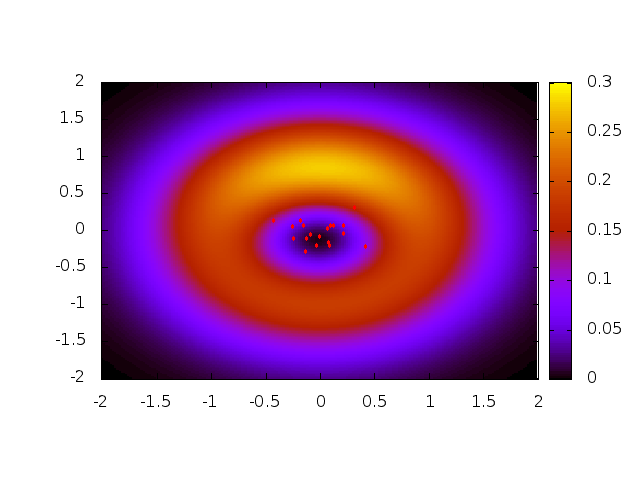
\includegraphics[scale=0.5]{deterioration1/deterioratedLandscape.png}
  }
  \caption{The result of basic deterioration scheme with CMA 
  applied to unimodal function: $f(X) = 2e^{-(x^2 +y^2)}$.
  Optics paramters: $minPts=20, \epsilon=0.4$, algorithm: SGA, iterationCount=1}
  \label{det1}
\end{figure}

\begin{figure}
  \centering
  \fbox{
    \includegraphics[scale=0.5]{deterioration3/fitnessLand.png}
  }
  \fbox{
    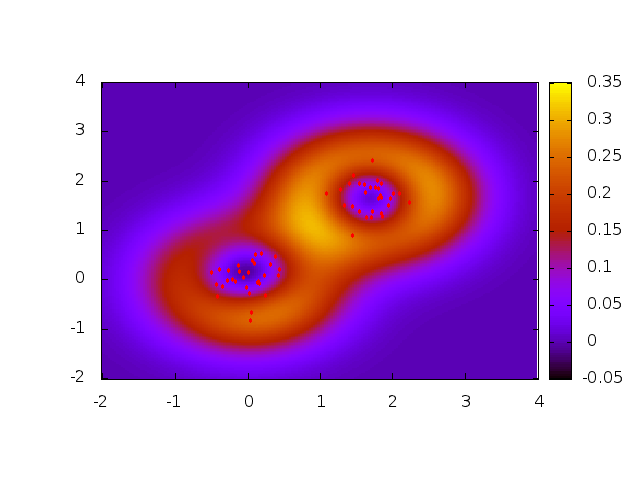
\includegraphics[scale=0.5]{deterioration3/deterioratedFitness.png}
  }
  \caption{The result of basic deterioration scheme with CMA 
  applied to bimodal function: $f(X) = e^{-(x^2 + y^2)}+1.4e^{-((x-1.7)^2 +
  (y-1.7)^2)}$. Optics paramters: $minPts=20, \epsilon=0.4$, algorithm: SGA, iterationCount=2}
  \label{det2}
\end{figure}

Figures $4.3$ and $4.4$ shows how much the algorithm benefit from using
the CMA algorithm. The plots show deterioration results applied to
functions from $4.1$ and $4.2$ without the CMA algorithm.

\begin{figure}
  \centering
  \fbox{
    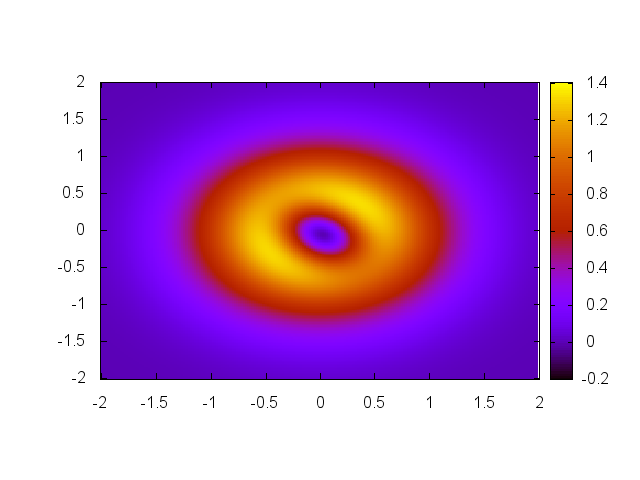
\includegraphics[scale=0.5]{deterioration4/result1_noCMA.png}
  }
  \caption{The result of basic deterioration scheme without CMA 
  applied to unimodal function from $4.1$. Optics paramters: $minPts=20,
  \epsilon=0.4$, algorithm: SGA, iterationCount=2. We may see that the 
  overall landscape decreases only by $30$ percent, while using CMA
  gives us $85$ percent of decline.}
  \label{det3}
\end{figure}

\begin{figure}
  \centering
  \fbox{
    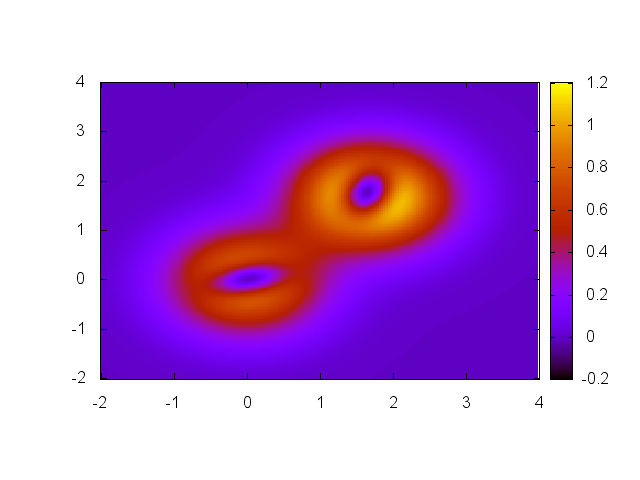
\includegraphics[scale=0.5]{deterioration4/result2_noCMA.png}
  }
  \caption{The result of basic deterioration scheme without CMA 
  applied to bimodal function from $4.2$. Optics paramters: $minPts=20,
  \epsilon=0.4$, algorithm: SGA, iterationCount=2. We see $25$ percent
  of deterioration, while CMA gives us $78$ percent when applied to the same
  case.}
  \label{det3}
\end{figure}

